\documentclass[sigconf,review,anonymous]{acmart}
\let\Bbbk\relax
\acmConference[ESEC/FSE 2023]{The 31st ACM Joint European Software Engineering Conference and Symposium on the Foundations of Software Engineering}{11 - 17 November, 2023}{San Francisco, USA}
% The preceding line is only needed to identify funding in the first footnote. If that is unneeded, please comment it out.
%% Use macros

%%% macros.tex
%%% Import packages, define utility commands and define macros
%%% Version 1.2.0

%%%----------
%%% Imports

%%% Text Formatting
\usepackage{microtype}
\usepackage{xspace}
\usepackage{xcolor}
\usepackage{graphicx}
\usepackage[normalem]{ulem} % normalem do not replace \emph to underline
\usepackage{amsmath}
\usepackage{enumitem}

%%% Reference, Citation and Link
\usepackage{hyperref}
%\usepackage{url}
\usepackage{breakurl}
%\usepackage{cite}

%%% Tables
\usepackage{booktabs}
\usepackage{multirow}
\usepackage{makecell}
\usepackage{ragged2e}

%%% Plots
\usepackage{caption}
%\usepackage{subcaption}
%\usepackage{subfloat}
%\usepackage{wrapfig}
\usepackage{subfig}

% Code
\usepackage{listings}

% Tikz Figs
\usepackage{tikz}
%\usepackage{pgf-umlsd} % for flow diagram
\usetikzlibrary{calc}
\usetikzlibrary{shapes.geometric}
\usetikzlibrary{decorations.pathreplacing}
\usetikzlibrary{positioning}
%\usetikzlibrary{shapes}

%%% Miscellaneous
%\usepackage{flushend} % balance the end of double column document
\usepackage{datetime} % for getting current date time

%%%----------
%%% Utility Commands
\newcommand{\XSpace}[1]{}
\newcommand{\XComment}[1]{}
\newcommand{\Fix}[1]{\textcolor{red}{#1}}
%\newcommand{\CR}[2]{\textcolor{blue}{#1}\textcolor{brown}{\sout{#2}}}
\newcommand{\CR}[2]{#1}
\newcommand{\EditAdd}[1]{\textcolor{green}{[#1]}}
\newcommand{\EditRm}[1]{\textcolor{red}{[\sout{#1}]}}
\newcommand{\EditMod}[2]{\textcolor{red}{[\sout{#1}]}\textcolor{green}{[#2]}}
\newcommand{\DefMacro}[2]{\expandafter\newcommand\csname rmk-#1\endcsname{#2}}
\newcommand{\UseMacro}[1]{\csname rmk-#1\endcsname}
\newcommand{\CfgStmtTableCaptionVSpace}{-5pt}
\newcommand{\ResultTableCaptionVSpace}{-5pt}
\newcommand{\AblationResultTableCaptionVSpace}{-5pt}

\newcommand{\jl}[1]{\textcolor{magenta}{JL: #1}}

\newcommand{\MyPara}[1]{\vspace{0pt}\noindent\textbf{#1}.}
\newcommand{\MyParaOnly}[1]{\noindent\textbf{#1}}
\newcommand{\reducedstrut}{\vrule width 0pt height .9\ht\strutbox depth .9\dp\strutbox\relax}
\newcommand{\InputWithSpace}[1]{\bgroup\def\arraystretch{1.2}\input{#1}\egroup}
\newcommand{\Code}[1]{{\ifmmode{\mathtt{#1}}\else$\mathtt{#1}$\fi}}
\newcommand{\CodeIn}[1]{{\ifmmode{\mathtt{#1}}\else$\mathtt{#1}$\fi}}
\newcommand{\ColorBack}[1]{%
  \begingroup
  \setlength{\fboxsep}{0pt}%
  \colorbox{purple!20}{\reducedstrut#1\/}%
  \endgroup
}

% for table headers
\newcommand{\specialcell}[2][c]{%
  \begin{tabular}[#1]{@{}c@{}}#2\end{tabular}}
\newcolumntype{R}[1]{>{\RaggedLeft\arraybackslash}p{#1}}
\newcolumntype{L}[1]{>{\RaggedRight\arraybackslash}p{#1}}
\def\clap#1{\hbox to 0pt{\hss#1\hss}}

%%% TEXT
%% \newcommand{\Title}{Naturalness of Hardware Designs}
%% \newcommand{\Title}{On the Naturalness of Hardware Designs}
\newcommand{\Title}{Programming Language Representation with Semantic-level Structure}

\newcommand{\TreeSitterURL}{https://github.com/tree-sitter/tree-sitter}

% Sorted alphabetically, ignoring case
\newcommand{\OurModelName}{Fuzz-CHECKLIST\xspace}
\newcommand{\Cfg}{CFG\xspace}
\newcommand{\lm}{langugae model\xspace}
\newcommand{\lms}{langugae models\xspace}
\newcommand{\Lm}{Langugae Model\xspace}
\newcommand{\dl}{deep learning\xspace}
\newcommand{\Dl}{Deep Learning\xspace}
\newcommand{\ml}{machine learning\xspace}
\newcommand{\ML}{Machine Learning\xspace}
\newcommand{\Trsfm}{Transformer\xspace}
\newcommand{\nlp}{nlp\xspace}
\newcommand{\Nlp}{NLP\xspace}
\newcommand{\Sw}{Software\xspace}
\newcommand{\sw}{software\xspace}
\newcommand{\se}{software engineering\xspace}
\newcommand{\Se}{Software Engineering\xspace}
\newcommand{\ho}{hold-out\xspace}
\newcommand{\sota}{state-of-the-art\xspace}
\newcommand{\ie}{i.e.\xspace}
\newcommand{\etal}{et al.\xspace}

\newcommand{\nn}{neural network\xspace}
\newcommand{\Bert}{BERT\xspace}
\newcommand{\Roberta}{RoBERTa\xspace}

%% Table
\newcommand{\tStatement}{\textbf{Statement Types}}
\newcommand{\tModel}{\textbf{Models}}
\newcommand{\tMetric}{\textbf{Metrics}}


%% Fig Caption
\newcommand{\PythonIntroExampleFigCaption}{
    An example \Py code snippet(\ref{fig:PythonCodeExample}) and
    its \Ast(\ref{fig:PythonAstExample}).\label{fig:PythonIntroExample}}
\newcommand{\CfgFigCaption}{Control-flow graph of code in
Fig~\ref{fig:PythonCodeExample}.\label{fig:PythonCfgExample}}
\newcommand{\PythonMotExampleFigCaption}{
    A motivational example \Py code snippet.\label{fig:PythonMotCodeExample}}
\newcommand{\MotCfgFigCaption}{Control-flow graph of code in
Fig~\ref{fig:PythonMotCodeExample}.\label{fig:MotCfgExample}}
\newcommand{\CodeExampleFigCaption}{Example code snippets predicted
from \graphcodebert and \CfgUndirDistnodeModel on \ctr task
(\ref{fig:TranslationCodeExample} and \cref task (\ref{fig:RefinementCodeExample})}


%% Table Caption
\newcommand{\CfgStmtTableCaption}{List of statement used for building \Cfg.\label{table:CfgStmt}\vspace{-5pt}}
\newcommand{\ResultTableCaption}{Results on \Nlp tasks
of \Ccd, \Ctr, \Cref repectively.\label{table:Result}\vspace{-5pt}}
\newcommand{\AblationResultTableCaption}{Results of ablation study
of \Cfg node type embedding on \Nlp tasks of \Ccd, \Ctr, \Cref repectively.\label{table:AbResult}\vspace{-5pt}}


%%% NUMBRERS
%% \input{tables/cfg-stmt-numbers}
%% \input{tables/results-numbers}


\begin{document}

\def\BibTeX{{\rm B\kern-.05em{\sc i\kern-.025em b}\kern-.08em
    T\kern-.1667em\lower.7ex\hbox{E}\kern-.125emX}}


\title{\tool{}: Specification- and Syntax-based Automated Testing Linguistic Capabilities of NLP Models}

%% Abstract
\begin{abstract}
  \Nlp (NLP) technique has become one of the core techniques for
  developing text  analytic applications.  These applications need to achieve high
  reliability to be useful in practice.  The trustworthiness of the NLP applications is often obtained by measuring the accuracy of
  the applications on holdout datasets. However, evaluating NLP on the accuracy of the holdout datasets is limited in validating its overall
  quality because these datasets are often not
  comprehensive. To address this limitation, evaluating an NLP model on
  task-specific behaviors defined on linguistic
  capabilities has been introduced. However, such evaluation relies on manually
  created test cases, and  is still limited to measure the model
  performance on limited datasets. In this work, we introduce \tool,
  an NLP model testing infrastructure.  Given a linguistic capability that users want to evaluate for a NLP model, \tool finds suitable seed inputs
  from existing datasets, generates sufficient number
  of new test inputs by expanding the seed inputs based on their \cfg
  (CFG).  We evaluate \tool by showing that it can generate test cases that are more diverse than an existing approach.
  We also show that \tool facilitates
  identification of critical failures and its origins in the NLP models
  for the \sa task.
\end{abstract}

% \begin{abstract}
%   \Nlp (NLP) technique\jl{technique, model, application?} becomes one of the core techniques for developing
%   text analytics applications.  For developing the NLP applications,
%   the applications are required to achieve high reliability before they
%   go to market\jl{<-simplify the sentence}.  The trustworthiness of the prevalent NLP
%   applications is obtained by measuring the accuracy of the
%   applications on test dataset.  However, evaluating NLP on
%   testset \jl{does with held-out accuracy??} is limited to show its quality
%   because the test datasets are often not comprehensive \jl{what does it mean?}. While the behavioral testing over multiple general linguistic capabilities are
%   employed, it relies on manually created test cases, and is still
%   limited to measure its comprehensive performance for each linguistic
%   capability \jl{does not make sense in terms of story telling}. In this work, we introduce \tool, an NLP model
%   testing methodology. Given a linguistic capability, The
%   \tool finds relevant testcases to test the linguistic
%   capability from existing datasets as seed inputs, generates
%   sufficient number of new test cases by fuzzing the seed inputs based
%   on their \cfg (CFG) \jl{<-long sentence}. We illustrate the usefulness of the \tool by showing input diversity and identifying
%   critical failures in \sota models for NLP task. In our experiment,
%   we show that the \tool generates {} more test cases with {}
%   higher diversity, and finds {} more bugs. \jl{describe what lc is about in a sentence} \jl{need to mention the result with numeric values}
  
% \end{abstract}


%% \title{\tool{}: Specification- and Syntax-based Automated Testing Linguistic Capabilities of NLP Models}
\maketitle

%% Contents
\section{Introduction}
\label{sec:intro}

%% [Thursday 3:01 PM] Yang, Wei

%% 1. existing NLP testing practice.

%% 2. Limitation in three perspectives:
%% (i) automated input generation,
%% (ii) test oracle (of generated input),
%% (iii) metrics/capabilities to debug the issues

%% 3. Issues with existing techniques: cannot satisfy all three requirements. Give some example, checklist (ii) and (iii), adversarial
%% testing (i) (ii) ....

%% 4. To address the limitation of existing work, we propose....

%% 5. insight that enable the three requirements


In the early stage of the software development process, automated
software testing and debugging can identify and fix
defects. Therefore, effective software testing assures software
quality, and it meets needs of the end user. Nowdays, software at work
has elements of \ml (ML). Especially, \Nlp (NLP) applications in
software are growing exponentially. Therefore, as quality assurance of
software is an essential process in the software development
processes, trustworthiness in quality of NLP application has become an
important component for its practical use in real world.
%% \sw{Should we lead with this paragraph? We are talking about
%%   functional testing here but next we say NLP uses
%%   train-validation-test.}
Traditionally, the prevalent models of NLP are evaluated via
train-validation-test splits. Training and validation set are used to
train the NLP models, and the test set, also named as \ho set, is used
for testing the trained model. Meanwhile, the model performance is
estimated into numbers used as performance metric. Especially,
accuracy, the fraction of model output that the model correctly
predicts, is the most widely the performance metric for classification
models. Accordingly, a model is considered better if it has higher
accuracy than another model.

Despite its simplicity and usefulness, there are several limitations
for the prevalent testing paradigm: First, the testing paradigm mostly
requires manual work for collecting and generating the data. The
manual work is costly with respect to time consumption and its impact
on market price. Therefore, it necessitates automated data generation
for improving model testing approach. Second, this testing paradigm
often overestimates the model performances from the \ho
set~\cite{patel2018mlevalforsoftware, recht2019imagenetbias,
  marcoACL2020checklist}.
%% \sw{Not sure what overestimate means here}
The overestimation comes from the discrepancy between distribution of
data collected and actual distribution in real world.  Oftentimes, the
\ho dataset is not representative and it is likely to introduce
specific biases. In addition, the inconsistency between test input and
its oracle causes biases. Such biases increase the discrepancy of
distribution between the dataset and real-world data. Consequently,
representiveness of the test data is required for testing approach.
Not only that, forced aggregation static into a single number such as
average makes user to difficult to localize and fix the bug found in
\ho set. Therefore, making this testing method fails to validate model
behaviors resulting in localization of the causes of the inaccuracy at
a high. In cost~\cite{wu2019errudite}. Therefore behavioral testing
approach provides the better ability to examine the inaccuracy and
find the bugs in the model.

To address these challenges, several approaches have been proposed to
evaluate different aspects of the NLP models, such as robustness on
adversarial examples \cite{ribeiro2018sear,belinkov2018breaknmt,
  rychalska2019wildnlp,iyyer2018adversarial}, model coverage
\cite{rottger2020hatecheck}, and fairness
\cite{prabhakaran2019fairness,rottger2020hatecheck}. In addition,
Ribeiro~\etal introduced \Cklst, a behavioral testing framework for
evaluating NLP model on multiple linguistic
capabilities~\cite{marcoACL2020checklist}. \Cklst defines
task-relevant linguistic capabilities and generates testcases for each
\lc. In spite of their effectiveness, they have limitations with
respective to model evaluation. For example, Testing model coverage
only shows model behaviors, but not the model performance on existing
testing set. The fairness and robustness testing only focus on only
one model capability resulting in its limited comprehensiveness. In
addition, \Cklst relies on manually generated input templates; thus,
the template generation requires manual work, and it needs to be
preset before test data generation. Consequently, the templates
becomes distributed in limited range of their structure. It restricts
its ability to comprehensively test the linguistic capabilities.

Despite the limitations, \Cklst approach of testing the linguistic
capabilities is a promising direction. Each \lc explains the
functionality of the input and output behavior for the NLP model under
test. Typically, it describes certain type of input and outputs
observed in real world for the target NLP task ranging from simple to
complicated behaviors so that they are able to evaluate the NLP model
comprehensively. For exmaple, a linguistic capability of ``Negated
neutral should still be neutral.'' measures how accurately the \sa
model understands the negative neutral input as an neutral
sentiment. Therefore, it requires the \sa model to output neural
sentiment on the negated neutral input.  Such methodology of
evaluation on the specified functionalities avoids the overestimation
of the model performance as it equivalently measures the model
performance on each functionality, and the separate model performance
explain distribution of the performance over the linguistic
capabilities. In the end, it provides not only the overall model
performance, but also the malfunction facets of the model.

To address the limitations of existing works, we present \tool, an
automated NLP model evaluation method for comprehensive behavioral
testing of NLP models on \sa task. We first address increasing input
representiveness. Compared with templates used in \Cklst, \tool
instead establishes input requirement for evaluating a linguistic
capability and finds suitable inputs that meet the requirement from
existing public dataset. In this process, \tool applies the fuzzing
testing principle to generate inputs by mutating the selected inputs
as seed inputs. Fuzzer in \tool first expands seed input grammar
structures and determines its available \pos to maintain structural
naturalness. After that, to hold contextual naturalness of the mutated
inputs, the fuzzer completes the expanded new structures via
data-driven context-aware word suggestion. Additionally,
sentiment-independent words in the inputs are replaced with rule-based
word suggestion. Further, we address the manual input generation
process by automating the process mentioned above. Lastly, we adopts
behavioral model testing method by introducing multiple behavior of
linguistic capabilities on \sa task and generating inputs relevant to
each linguistic capability.

We demonstrate its generality and utility as a NLP model evaluation
tool by evaluating well-known \sa models: \Bert~\cite{devlin2019bert},
\Roberta~\cite{liu2019roberta} and \Dbert~\cite{sanh2019distilbert}.
We show that ...

\section{Background}
\label{sec:background}

In this section, we provide a brief background of \Cklst's \cite{marcoACL2020checklist} approach of test case generation
 via an example.
%  Quality of software is verified by ensuring
% the proper working of all functionalities without knowing the internal
% workings of the software. Knowing performances of model on the
% multiple functionalities provides users with better understanding and
% debugging the software. The same principle applies to the NLP model.
% Traditional NLP model evaluation relying on a test set lacks the
% specification of model functionality. However, in NLP domain, there
% are many phenomena on linguistic input such as negation, and
% questionization. Given a NLP task, the phenomena determine
% task-relevant output. Traditional evaluation method neglects them;
% thus, it becomes less efficient to detect and analyze which aspect the
% model yields unexpected outcome.
\Cklst
introduces task-dependent \lcs for monitoring model performance on
each \lc. It assumes that the linguistic phenomena can be represented
in the behavior of the model under test, because each linguistic capability specifies the desired behavior between model inputs and outputs. For each \lc, \Cklst manually creates
test case templates and generates sentences by filling in the values of
each placeholder.

\begin{figure}[t]
 \centering
 \lstinputlisting[language=python-pretty]{code/checklist_template2.py}
 \vspace{-10pt}
 \caption{\CklstTemplateFigCaption}
 \vspace{-10pt}
\end{figure}

We show an example of \Cklst templates in
Figure~\ref{code:TempEx}. These templates are used for
evaluating the \sa model on the linguistic capability of \SareqExThree.
For the templates defined
at lines~\ref{code:tempex:template:1} to \ref{code:tempex:template:2}, they
have placeholders such as ${it}$, ${air\_noun}$, ${pos\_adj}$. Values
for the placeholders are defined at
lines~\ref{code:tempex:airnoun:1} to~\ref{code:tempex:negadj:2}.
For each template, \Cklst fills in all the combinations of the
values of placeholders to generate sentences under this \lc.
For example, sentences such as ``The flight is good'' and ``That
airline was happy'' are generated using the template at line 10.

Despite the simple approach used for test case generation, \Cklst has
limitations. First, it relies on manual work for defining template
structure and its placeholder values, making the test case
generation a costly process. Moreover, such
manual work generates a limited number of templates, produces similar test cases, and induces bias in the test cases. These limitations motivated the design of our approach.
\section{Technique and implementation}
%% \label{sec:approach}

\begin{figure*}
  \centering
  \includegraphics[scale=0.5]{figs/overall.pdf}
  \vspace{-5pt}
  \caption{\OverallModelFigCaption}
  \vspace{-10pt}
\end{figure*}

\Model generates input sentences with the following phases illustrated
in \ref{fig:OverallModel}: 1. search phase searches seed sentences according to
its requirement of \lc, 2. seed parsing phase parses the found seed
sentences and extract their \cfg, 3. reference phase collects large
corpus, 4. syntax expansion identification, and 5.sentence expansion
and generation. In this section, we provide more details on each phase.

\subsection{Search phase}
The search phase in \Model searches and samples subset of sentences in the
dataset that meets the requirement extracted from each linguistic
capability. Each linguistic capability represents performance of \nlp
task on specific input domain

requires certain format of sentences


%\section{Research questions for evaluation}
\label{sec:rq}

section{Experiment}
\label{sec:experiment}
%
In this section, we present experiments to evaluate the effectiveness
of our proposed evaluation methodology. In particular, we address the
following research questions:

\begin{enumerate}[label=\textbf{RQ\arabic*}]
\item \label{rq:one}: How effective is our proposed evaluation model
  for finding failures given a linguistic capability?
\item \label{rq:two}: How effective is our proposed model for
  generating diverse test cases? % self bleu score
\item \label{rq:three}: How effective is test cases generated from our
  proposed model for detecting diverse type of errors? % retraining
  acc score
\item \label{rq:four}: How effective is our new test case generation
  using \cfg expansion? % ablation study
\end{enumerate}

For answering \ref{rq:one} and \ref{rq:two}, we generate test cases
and use them for evaluating model on linguistic capabilities. In this
experiment, We assess the ability to find failures by anlyzing model's
performance on the generated test cases. We also measure the diversity
among the generated test cases using similarites among them. Next, we
answer \ref{rq:three} by retraining \sa model with generated test
cases and measuring performances. The idea behind this is that more
comprehensive inputs becomes closer to real-world distribution and
addresses more type of errors.  Therefore, it leads to improve the
model performance. In this experiment, We retrain the model and
compare performances of the retrained model. Not only that, we conduct
ablation study of \cfg expansion to understand the its impact in our
approach.

\subsection{Experiment Setup}
%
\MyPara{Seed Input Selection}
%
For each linguistic capability, we first search all sentences that
meet its requirement. Among found sentences, we randomly select 10
sentences due to memory constraint.

\MyPara{Word Sentiment}
%
we extract sentiments of words using the
\Swn~\cite{baccianella2010sentiwordnet}. The \Swn is a publicly
available lexical resource of words on Wordnet with three numerical
scores of objectivity, positivity and negativity. Sentiment word
labels from the scores are classified from the algorithm from Mihaela
\etal~\cite{mihaela2017sentiwordnetlabel}.

\MyPara{\Cfg Expansion}
%
We build a reference \Cfg of natural language from the English Penn
\Trb corpora~\cite{mitchell1993treebank,nltkTreebankCorporaWebPage}.
The corpus is sampled from 2,499 stories from a tree year \Wsj
collection The \Trb provides a parsed text corpus with annotation of
syntactic and semantic structure. In this experiment We implement the
\trb corpora available through \Nltk, which is a suite of libraries
and programs for \Nlp for English. In addition, we parse the seed
input using into its CFG using the Berkeley Neural
Parser~\cite{kitaev2018constituency, kitaev2019multilingual}, a
high-accuracy parser with models for 11 languages. The input is a raw
text in natural language and the output is the string representation of
parse tree. Next after comparing CFGs between reference and seed input,
we randomly select 10 expansions for generating templates due to
memory constraint.

\MyPara{Synonyms}
%
\Model searches synonyms of each token from synonym sets extracted
from \Wrdnt using \Spacy open-source library for NLP.

\MyPara{Models}
%
We evaluate the following \sa models via \Model:
\Bert~\cite{devlin2019bert}, \Roberta~\cite{liu2019roberta} and
\Dbert~\cite{sanh2019distilbert}. These models are fine-tuned on \Sstt
and their accuracies are \BertAcc, \RobertaAcc and \DbertAcc.

\MyPara{Retraining}
%
We retrain \sa models. we split \Model generated test cases into
train/validation/test sets with the ratio of 8:1:1. The number of
epochs and batch size for retraining are 1 and 16 respectively.

\section{Experimental Results}
\label{sec:result}

This section presents the experimental results and the answers to the RQs. 
More results are available at the \tool repository.\footnote{\href{https://github.com/csresearcher27/s2lct_project}{https://github.com/csresearcher27/s2lct$\_$project}} 
% \sw{@Jaeseong: footnote typically goes after punctuation, without space. I fix these; just wanted to let you know.}

\InputWithSpace{tables/test-results-all-table}
% \InputWithSpace{tables/test-results-table}
% \InputWithSpace{tables/test-results-3-50-table}
% \InputWithSpace{tables/test-results-3-100-table}
% \InputWithSpace{tables/test-results-3-200-table}
\InputWithSpace{tables/test-results-hs-table}

\begin{figure}
    \centering
    \includegraphics[width=0.35\textwidth]{figs/pdr-selfbleu-agg-lc-task-agg-lineplot.eps}
    \vspace{-3mm}
    \caption{\PdrSelfbleuFigCaption}
\end{figure}

\begin{figure}
    \centering
    \includegraphics[width=0.3\textwidth]{figs/pdr-selfbleu-ablation-lc-task-agg-barplot.eps}
    \vspace{-3mm}
    \caption{\PdrSelfbleuBarplotFigCaption}
\end{figure}

\InputWithSpace{tables/mtnlp-comp-table}
\InputWithSpace{tables/adv-comp-table}

% \begin{figure}%
%     \centering
%     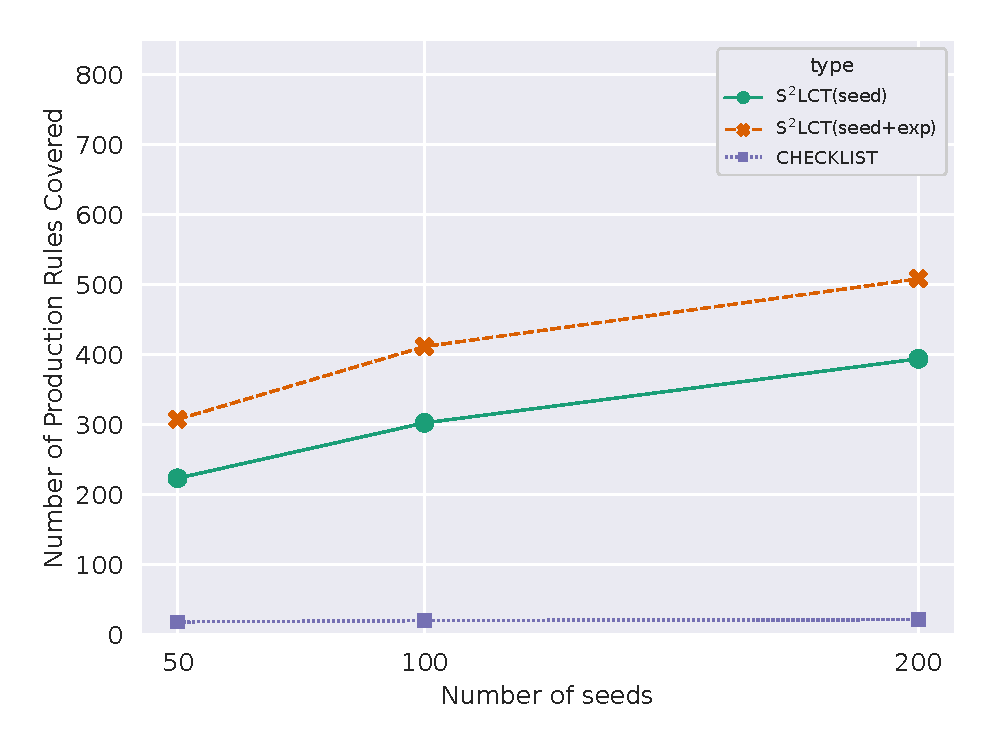
\includegraphics[width=0.35\textwidth]{figs/pdr-agg-lineplot.eps}
%     \caption{\PdrFigCaption}
% \end{figure}


% \begin{figure}%
%     \centering
%     \subfloat[][\centering\SelfbleuFigCaption]{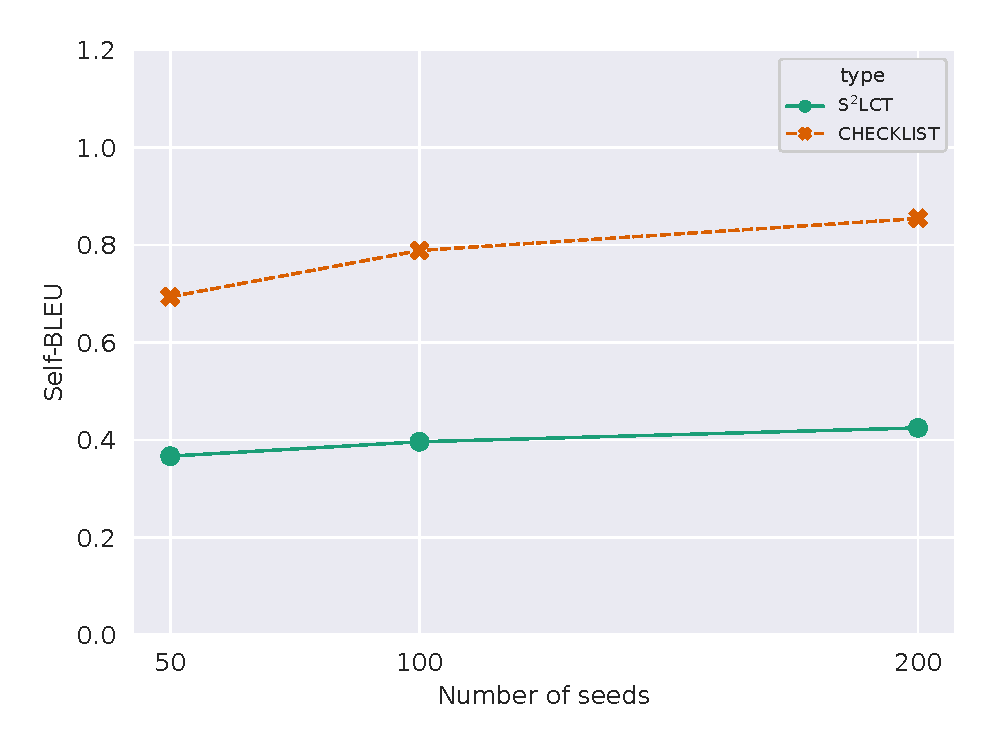
\includegraphics[width=0.35\textwidth]{figs/selfbleu-agg-sample-lineplot.eps}}%
%     \qquad
%     \subfloat[][\centering\PdrFigCaption]{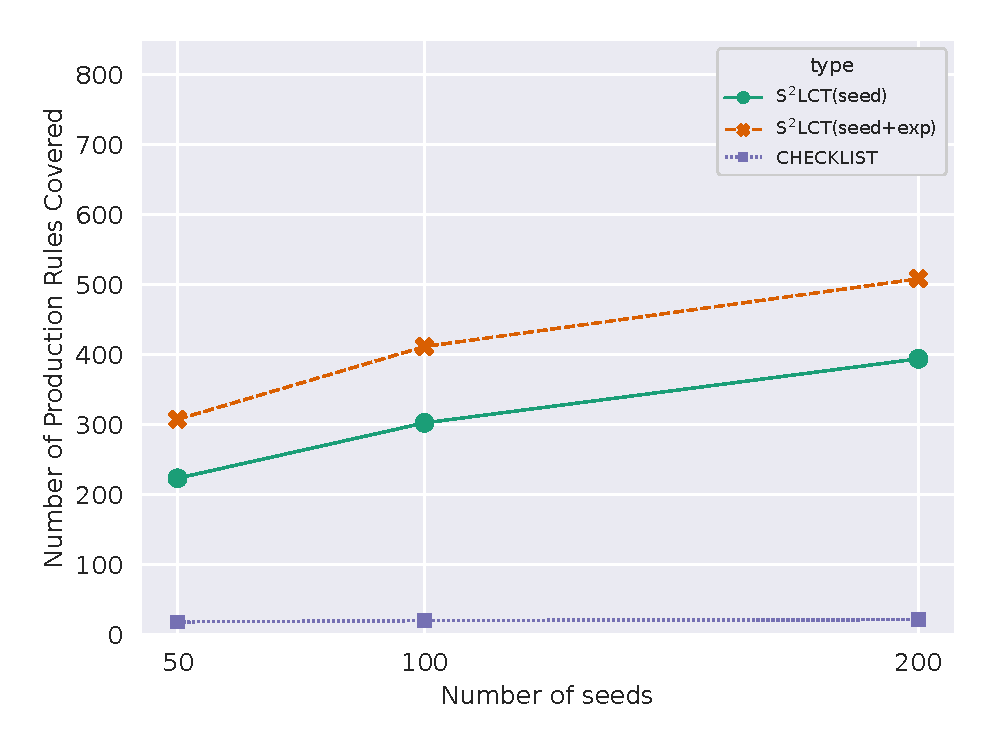
\includegraphics[width=0.35\textwidth]{figs/pdr-agg-lineplot.eps}}
%     \caption{\FailModelsFigCaption}
% \end{figure}

% \begin{figure}%
%     \centering
%     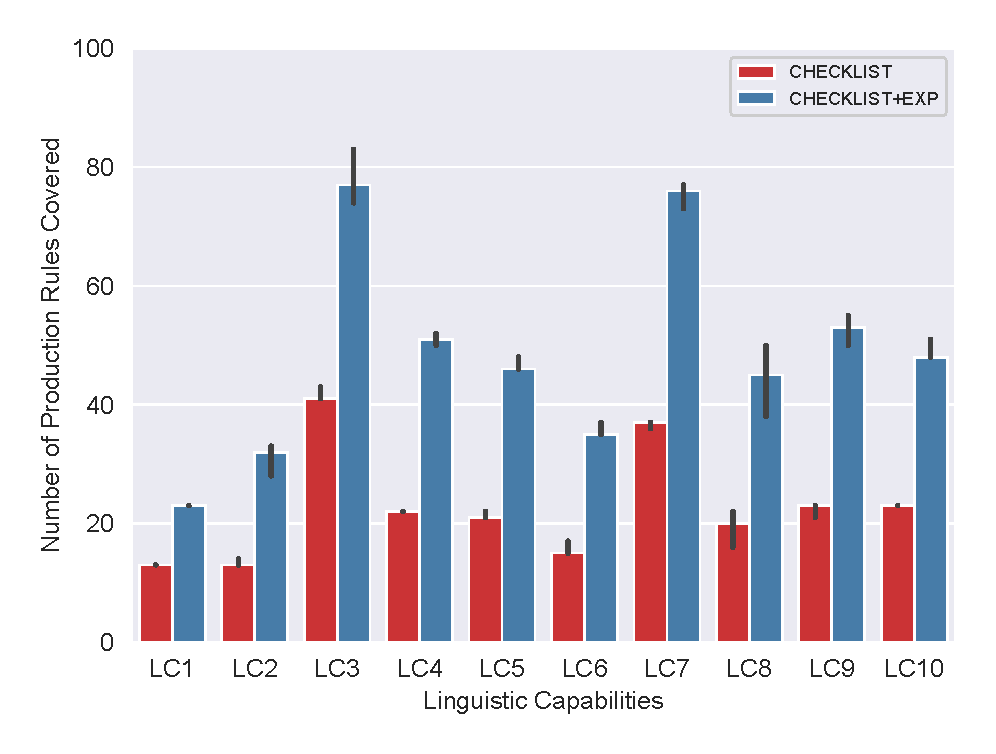
\includegraphics[width=0.4\textwidth]{figs/pdr-checklist-barplot.eps}
%     \caption{\PdrBarplotFigCaption}
% \end{figure}

% \begin{figure}%
%     \centering
%     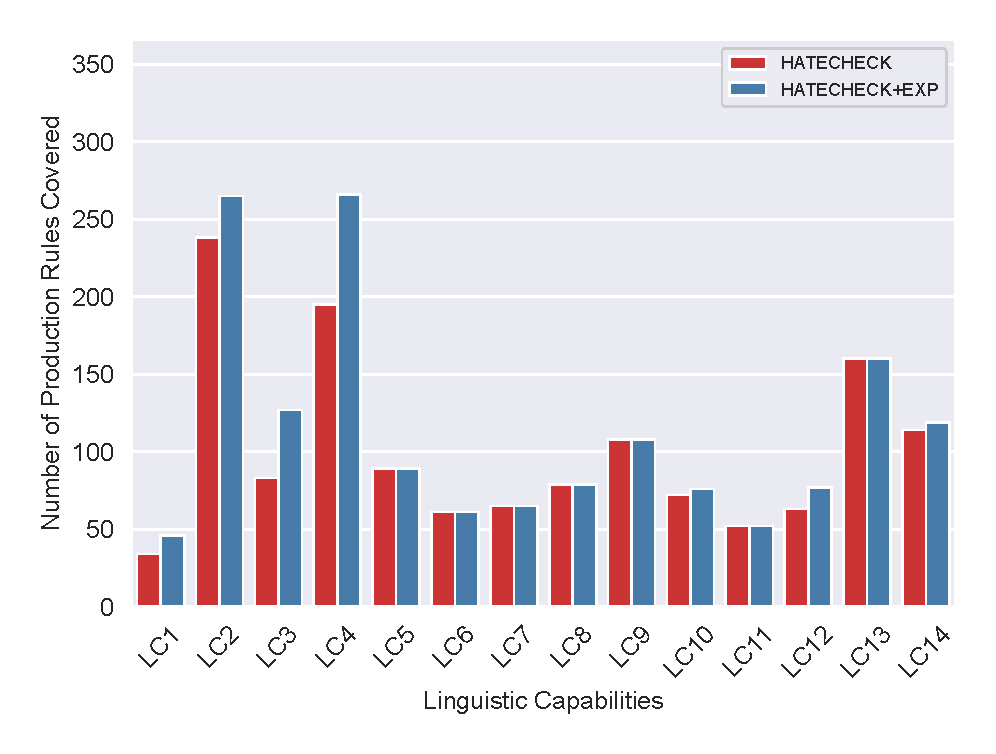
\includegraphics[width=0.45\textwidth]{figs/pdr-hatecheck-barplot.eps}
%     \caption{\PdrBarplotHsFigCaption}
% \end{figure}

% \begin{figure}%
%     \centering
%     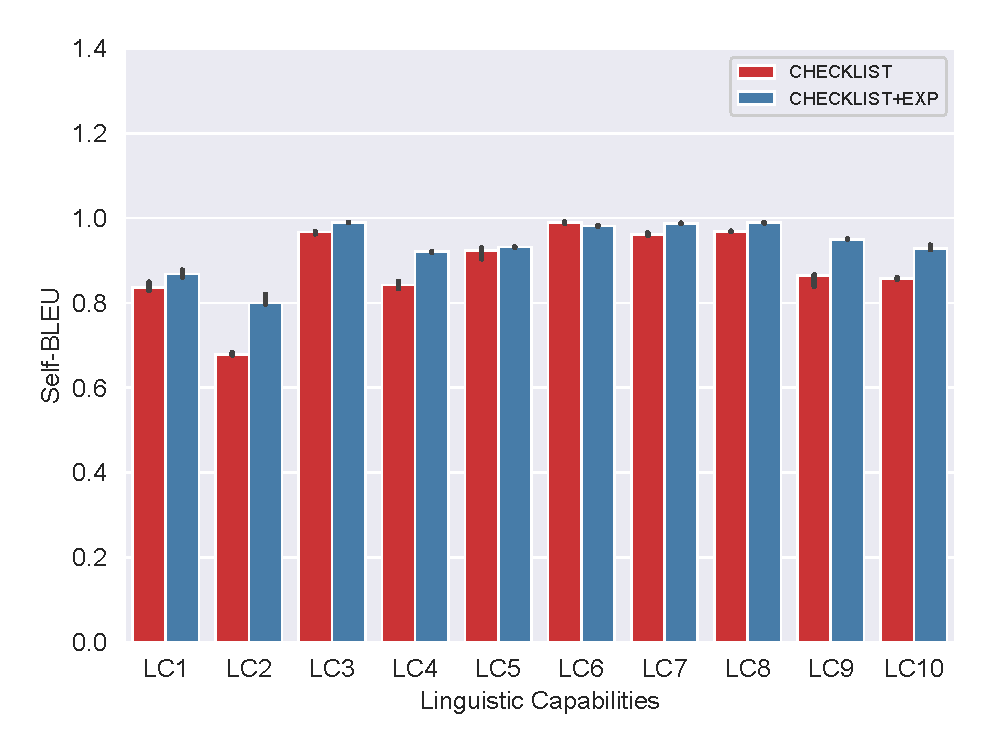
\includegraphics[width=0.4\textwidth]{figs/selfbleu-checklist-barplot.eps}
%     \caption{\SelfbleuBarplotFigCaption}
% \end{figure}

% \begin{figure}%
%     \centering
%     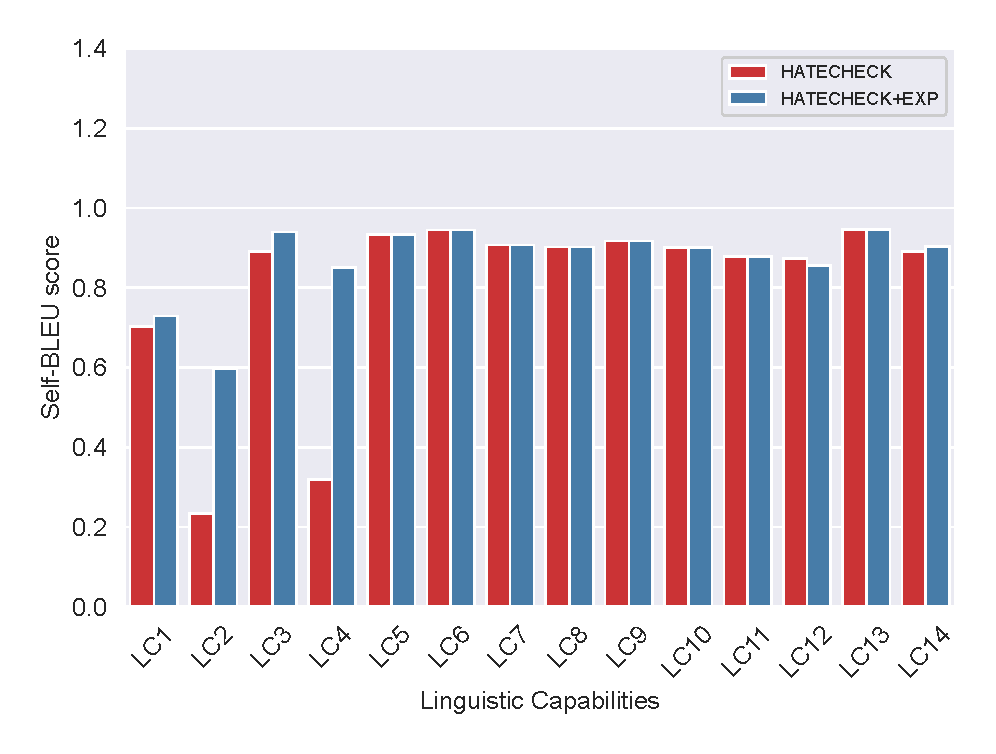
\includegraphics[width=0.45\textwidth]{figs/selfbleu-hatecheck-barplot.eps}
%     \caption{\SelfbleuBarplotHsFigCaption}
% \end{figure}

% \begin{figure}%
%     \centering
%     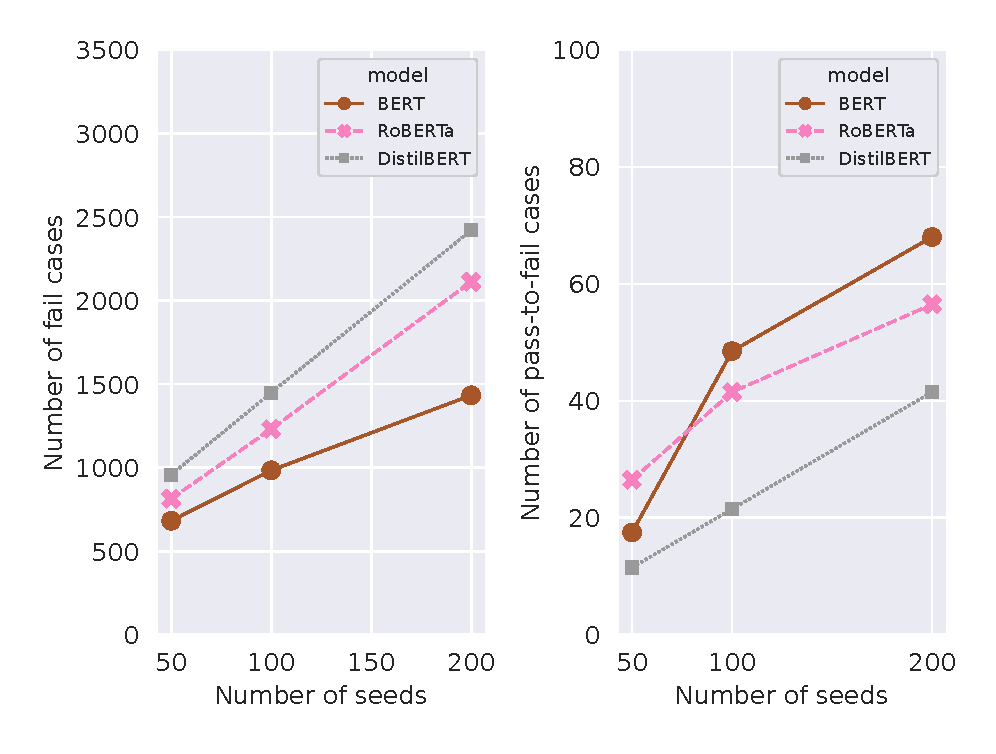
\includegraphics[width=0.35\textwidth]{figs/numfail-pass2fail-agg-lineplot.eps}
%     \caption{\FailModelsFigCaption}
% \end{figure}

% \begin{figure}%
%     \centering
%     \subfloat[][\centering\NumFailModelsSubFigCaption]{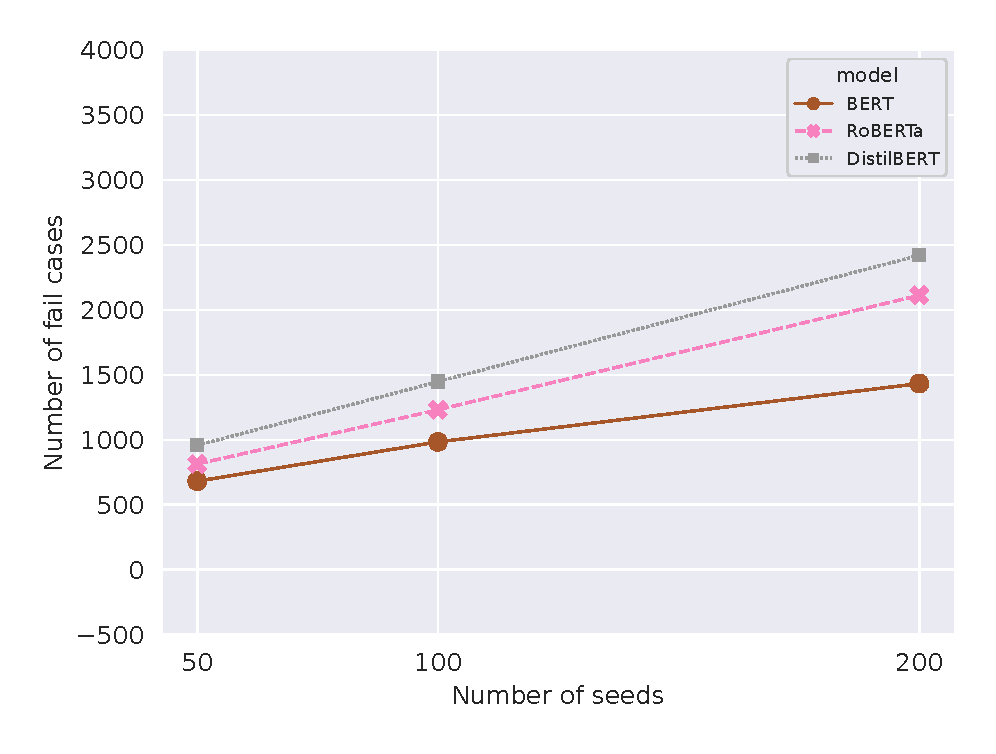
\includegraphics[width=0.35\textwidth]{figs/numfail-agg-lineplot.eps}}%
%     \qquad
%     \subfloat[][\centering\FailRateModelsSubFigCaption]{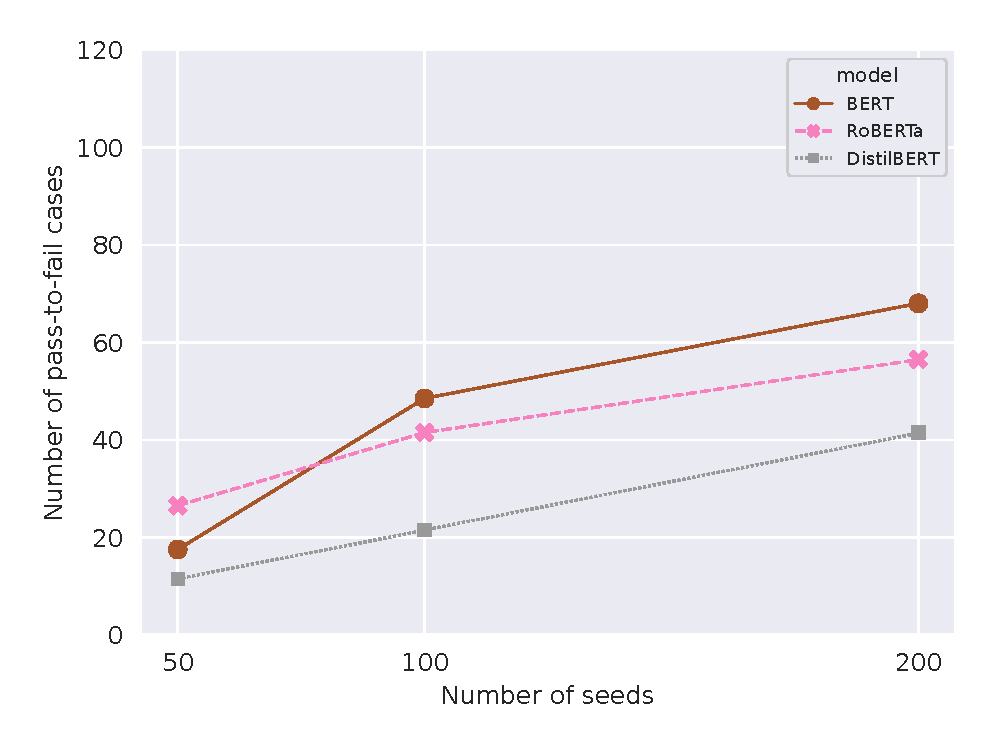
\includegraphics[width=0.35\textwidth]{figs/pass2fail-agg-lineplot.eps}}
%     \caption{\FailModelsFigCaption}
% \end{figure}

\subsection{\ref{rq:one}: Diversity}

% Our results show that \emph{\tool generated many test cases that the sentiment analysis models failed to predict the correct labels, and it produced significantly more diverse test cases than \Cklst did.}
Our results show that \emph{\tool produced test suites with significantly more diversity than \bls did.} 
% In this experiment, we show the test case diversity by comparing \selfbleu and \pdr metrics between \tool and capability-based testing \bls. In addition, we show increase in test case diversity by comparing \selfbleu and \pdr metrics between \tool using \Cklst and \hck as seeds and \Cklst and \hck themselves.

\MyPara{\selfbleu and \Pdr} 
Figure~\ref{fig:PdrSelfbleu} compares the \selfbleu and \pdr scores of the test suite generated by \tool in contrast to those of \Cklst and \hck.
The x-axis shows the sizes of the generated test suite, and the y-axis shows the metric scores.
% Median value of \selcbleu scores are computed from randomly sampled seeds over 3 trials for each \lc,
The figure displays the median \selfbleu and \pdr scores over all \lcs and 5 trials on the left and right, respectively. The results show that \tool's test suite is more diverse than the baselines', with significantly lower \pdr scores and significantly higher \selfbleu scores. This highlights the advantages of searching from a real-world dataset rather than relying on limited preset templates. Furthermore, using expanded sentences in \tool leads to lower \selfbleu and higher \pdr scores, demonstrating the syntax-based expansion of \tool improves sentence diversity.

Figure~\ref{fig:PdrSelfbleuBarplot} shows the \selfbleu and \pdr scores of test suites generated by baseline methods and their expanded versions using \tool. The x-axis shows the method name, and the y-axis shows the corresponding scores across all \lcs. The left sub-figure displays the \selfbleu scores, and the right sub-figure shows the \pdr scores. The results indicate that the expanded \Cklst and \hck achieve better \pdr scores than their original versions, demonstrating the effectiveness of \tool's syntax-based expansion module in increasing the diversity of the generated test suite. Additionally, the expanded \Cklst performs worse in terms of \selfbleu scores, while the expanded \hck has comparable scores to its original version.

Table~\ref{table:MtnlpComp} compares \tool's expanded \sents and \mtnlp for 100 randomly selected seeds. The first column lists the NLP task, and the second column displays the approaches for text generation. Columns 3-5 show the number of generated \sents, \selfbleu, and \pdr scores over 5 sampling trials. \tool generates more \sents than \mtnlp for all tasks and has higher \selfbleu and \pdr scores, demonstrating the effectiveness of \tool's syntax expansion in increasing test case diversity. \mtnlp sometimes fails to mutate seed \sents due to the unavailability of suitable human-related words for mutation.

Table~\ref{table:AdvComp} compares \tool-expanded \sents with adversarial text generation baselines from Section~\ref{sec:experiment_bl}. The first column shows the approach type and the second column shows the number of generated \sents using \tool and the baselines from 50 randomly selected seeds. The third and fourth columns show the \selfbleu and \pdr scores over 5 sampling trials. Results show that Alzantot~\etal~\cite{alzantot2018genadvexp} has the lowest \selfbleu scores, whereas \tool expansion achieves the highest scores in the number of generated \sents and \pdr, introducing various syntax components while maintaining text diversity.



% \paragraph*{\Pdr} Right in figure~\ref{fig:PdrSelfbleu} compares \pdr between the \tool seed sentences, \tool seed and expanded sentences, and the \Cklst test cases. The x-axis shows the sizes of random samples of \tool seed sentences, \tool seed and expanded sentences, and \Cklst test cases, and y-axis shows the \pdr scores. Median of the \pdr scores over all \lcs is shown in the right in the figure~\ref{fig:PdrSelfbleu}. The figure \ref{fig:PdrSelfbleu} shows that \tool seed and/or expanded sentences produce significantly higher \pdr scores than \Cklst test cases did. Also, more \tool seeds cover more production rules because of the increase in diversity obtained from more \tool seeds.

% Figure~\ref{fig:PdrBarplot, HsPdrBarplot} compares the \pdr between all \tool seeds and all \Cklst test cases for each \lc. The x-axis shows each one \lc, and the y-axis is the natural logarithmic scale of \pdr for these test cases.
% % \tool test cases are generated from randomly selected 50 seeds, and the median value over 3 trials for each \lc is reported.
% % It is observed that \tool covers significantly higher number of different syntactic production rules than \Cklst for all \lcs.
% We observed that \tool seeds cover significantly higher number of production rules in each \lc than all \Cklst test cases (ranging from 90 for LC1 to 8518 for LC8 for \tool seeds and from 13 for LC1 to 44 for LC3 for \Cklst seeds) in each \lc.
% % (ranging from 4.92 times to 20.38 times higher scores for LC7 and LC6 respectively) 

% Overall, the above results show that \tool test cases are significantly more diverse with regards to semantic and syntactic structure than \Cklst.


\begin{figure}
    \centering
    \includegraphics[width=0.5\textwidth]{figs/covergae.pdf}
    \caption{The coverage results of the generated test
      samples. \sw{Make the figures larger.}}
    \label{fig:coverage}
\end{figure}


Fig. \ref{fig:coverage} shows the coverage results of the generated
test samples, where the red line represents \tool and the black line
represents \Cklst.  Each column in Fig. \ref{fig:coverage} represent
the results for one NLP model, the first row is the \textit{BoundCov}
results and the second row is the \textit{SActCov} results.  From the
results, we make two observations observations. First, for \emph{all}
experimental settings (\eg NLP model, coverage metric), \tool achieves
high coverage than \Cklst. Recall that a higher coverage implies the
test case in the test suite is more diverse and rarely to have a
statistical distribution similar to the model training data. As a
result, a test suite with greater coverage complements the model
training data distribution (\ie hold-out testing data) better.  The
experimental results confirm that \tool can generate more diverse test
cases to complement the hold-out testing data for testing NLP models.
\sw{What does the growth trend in each figure indicate?} \sw{Does the
  absolute numbers or relative difference of the two lines on y axis
  mean anything concrete? E.g., how significant is the improvement in
  diversity?}

Another interesting finding is that for each NLP model, there is no
fixed relationship between \textit{BoundCov} and \textit{SActCov}. In
other words, while a test suite may produce higher \textit{BoundCov}
for some models, the same test suite may get higher \textit{SActCov}
for other NLP models.  Recall that \textit{BoundCov} measures both the
upper and lower corner neurons and \textit{SActCov} measures only the
upper corner neurons.  Such observation implies that the upper and
lower corner neurons are distributed unevenly, and measuring only one
of them is not enough.


\subsection{\ref{rq:two}: Effectiveness}
Our results show that \emph{\tool generates diverse test cases that expose classification errors in NLP models, outperforming the baselines.}
%Specifically, we compared the testing results of \tool with \Cklst for \sa and \hck for \hsd.

\MyPara{The Number of Test Cases}
Table~\ref{table:TestResultAll} and~\ref{table:TestResultHsd} present the results of our effectiveness metrics defined in Section \ref{sec:metric}.  For all \lcs, \tool generates a significant number of test cases, ranging from 70 on LC1 to 533,575 on LC8.
For LC1, LC2, LC4, and LC5, \tool generates fewer test cases than \Cklst because of the small number of seeds. However, the syntax-based sentence expansion phase generated 51 to 503 test cases. In Table~\ref{table:TestResultHsd}, \tool generates more test cases than \hck for every \lcs except LC11, indicating that \tool is more beneficial in generating a sufficient number of test cases. The results show that \tool generates many test cases in the NLP models that fail to predict the correct labels, providing further qualitative test cases than baselines for finding errors.

\MyPara{Fail Rate and Failed Cases}
Figure~\ref{table:TestResultAll} demonstrates that at least one model introduces a higher number of failed test cases on \tool test cases than \Cklst in 7 \lcs, and at least one model achieves a higher failure rate on \tool than on \Cklst in all other \lcs (ranging from 4.27\% to 99.64\%) except for LC8 and LC9. Additionally, in table~\ref{table:TestResultHsd}, we observe that every \lcs for \hsd has a higher number of failed test cases on \tool test cases than \hck, with the failure rate being higher for at least one model in every \lcs except for LC1 and LC5 (ranging from 1.89\% to 88.89\%). Based on these findings, we can conclude that \tool is more effective in generating test cases to identify  errors.

% \paragraph*{Failed Cases}
% Left in figure~\ref{fig:FailModels} compares the numbers of failed cases between \tool and \Cklst. 
% The x-axis shows the sizes of random samples of \tool seed sentences and CHECKLIST test cases, and y-axis shows the number of failed cases. Median number of failed cases from \sa models over \lcs is shown in left in figure~\ref{fig:FailModels}. We observed that \tool seeds introduce more failed cases than \Cklst test cases, and it shows the higher effectiveness of \tool test cases. In addition, it shows that more \tool seeds presents more failed cases, demonstrating the benefit of using more seeds when resource permits.

\MyPara{\Ptf Cases} We observed that many test cases failed in the expanded set but not in their corresponding seeds (as shown in the last column of Table~\ref{table:TestResultAll} and~\ref{table:TestResultHsd}). This type of error case ranges from 0 to 12,729 for \sa and from 0 to 4,365 for \hsd. These results demonstrate that the syntax-based sentence expansion phase effectively introduces more diverse sentence structures, which can potentially expose errors in NLP models that may not be evident in the original seed test cases.

\InputWithSpace{tables/manual-study-table}

\subsection{\ref{rq:three}:  Consistency}


Table~\ref{table:ManualStudy} shows the results of our consistency study. The first column lists the NLP tasks, and the second column distinguishes between seed and expanded sentences. The third column indicates the number of test cases used. Columns 4-6 present the scores of label consistency, LC relevancy, and expansion validity sentences, respectively. Our analysis shows that \emph{\tool generates test cases with high label consistency}, with scores of 0.83 for both seed and expanded test cases for \sa and 0.80 and 0.79 for seed and expanded cases, respectively, for \hsd, indicating that the test oracles constructed by \tool align with human sentiment labeling most of the time.
Moreover, the results show high expansion validity scores of 1.0 for \sa and 0.97 for \hsd, indicating that the tool effectively preserves the semantic meaning of seed sentences during the expansion process. The \lc relevancy score is presented in column 5 of Table \ref{table:ManualStudy}. The result shows that \emph{\tool generates test cases that are correctly categorized to the corresponding \lcs most of the time}. The \lc relevancy scores for the seed and expanded sentences are 0.92 and 0.84 for \sa and \hsd, respectively, achieving high agreement with human assessment. The fact that the expanded sentences generated by \tool have the same level of \lc relevancy as the seed sentences demonstrates that the syntax-based sentence expansion retains the \lcs.












\section{Application of \tool}
\label{sec:application}
% \item \label{rq:four}: \textbf{Usefulness of Test Inputs.} 

In this section, we showcase how \tool can be used in conjunction with explainable ML techniques to assist developers in identifying the root causes of bugs in \sa models.

\begin{figure*}
    \centering
    \includegraphics[width=0.7\textwidth]{figs/explain.pdf}
    \vspace{-4mm}
    \caption{Visualization of the buggy reason of two \tool generated test cases.}
    \label{fig:explain}
\end{figure*}


\MyPara{Experimental Process}
we conduct experiments to demonstrate that \tool can help developers understand the bugs in the NLP models.
Recall that \tool generates test cases by mutating seed sentences (\eg by expanding one token in the seed input). Still, it is unclear why mutating one token will cause the model to produce misclassified results.
We seek to help developers understand why such mutation will result in the misclassification. 
Existing work \cite{simin2020denas, lemna, lime} has demonstrated that the ML model prediction is dominated by a minimal set of input features (\ie tokens in input sentences). Motivated by such intuition, we identify a minimal set of input tokens that dominate the model prediction.

Formally, given a input sentence $x = [tk_1, tk_2, \cdots, tk_n]$, and the NLP model under test $f(\cdot)$, our goal is to find a masking template $T = [t_1, t_2, \cdots, t_n]$, where $t_i$ is 0 or 1, representing masking the $i^{th}$ token (\ie $tk_i$) in $x$ or not.
The template $T$ can mask some tokens in $x$ with attribute tokens, and the masked input has a high probability of retaining the original prediction $x$, denoted as
\begin{equation}
    P(f(T(x)) = f(x)) \ge P_{thresh}
    \label{eq:prob}
\end{equation}
To create such a template $T$, we first compute the contribution score of each input token using an existing explainable ML technique \cite{lemna}. We then begin with the full mask template (\ie, all tokens are masked); such full mask template definitely does not satisfy Equation \ref{eq:prob}.
We then iteratively shift one position from mask to non-mask based on the order of each token's contribution score, until the template $T$ satisfies Equation \ref{eq:prob}.
Because we iterate the size of the mask, the generated template $T$ will keep the minimum number of tokens in $x$. Moreover, since the input $x$ is an incorrect prediction, the generated template $T$ is likely to produce misclassification (i.e., the probability to be misclassified is larger than $P_{thresh}$).

\MyPara{Results} We generate a template that dominates the NLP model prediction to assist developers in understanding the false predictions. Figure \ref{fig:explain} shows the generated templates for two randomly selected seeds and their corresponding expanded test inputs.
The first example tests ``sentiments in (question, yes) form'' (LC9), and the second example tests ``negative positive with neutral content in the middle''  (LC7).
The first column shows the seed sentence, the second shows the expanded sentence, and the third shows each token's contribution score. The blue bar indicates the score for seed inputs, whereas the orange bar reflects the score for the expanded sentences.
We highlight the mutated token with yellow background and generated templates with red text. 

The results show that after mutating the seed sentence with one token, the token set that dominates the NLP model prediction has changed.
We can trace the root causes to the bias of the training data on the \lc under test; as a result, for the \lc under test, the model has a bias towards positive/negative for certain token sequence patterns. For example, LC9 has a bias toward the token sequence pattern that includes "maybe .... but ... even... yes". Thus, adding the token ``even" to the seed sentence will match one of those biased sequence patterns.
Sentences with such pattern in the training dataset are dominantly positive; thus, the models make the wrong decision on the sentence with ``even'' as positive. 
The visualization of each token's contribution score in the third column confirms our observation. Once ``even'' is added, scores of other tokens such as ``but'' and ``yes'' all change from negative to positive.
To fix the issue for LC9, we need to add more negative training samples with the format of ``maybe . .. but ... even ... yes''.
%he experimental results in Fig. \ref{fig:explain} illustrate that \tool can help developers to understand the buggy reason of the misclassification go no在,
\section{Threats to Validity}
\label{sec:threats}

Use of publicly available datasets poses an external validity threat
with respect to the generalizability of our results. We implemented
domain-spefic knowledge on publically available word sentiments
dataset~\cite{baccianella2010sentiwordnet}. We also constructed
reference CFG from publically available corpus dataset
\cite{mitchell1993treebank, nltkTreebankCorporaWebPage}. The dataset
used in our study might not be completely representative of all
English grammatical structures and English word sentiments. We
mitigate this threat by observing that they are widely used in NLP
domain~\cite{husnain2021swnvalidity} and reviewed each script and the
output logs.


\section{Related Work}
\label{sec:related}

\MyPara{NLP Testing.}
%
With the increasing use of NLP models, evaluation of NLP models is
becoming more important. Apart from the task accuracy based testing
scheme, recent works have also considered model robustness as an
aspect for model evaluation. Belinkov
\textit{\etal}~\cite{belinkov2018breaknmt} aims to fail neural machine
translation model by intentionally introducing noise in the input
text.Pinjia
\textit{\etal}~\cite{pinjia2020structinvtestingnmt,pinjia2020testnmtrt}
measures the robustness by assuming syntatic and semantic relation
between input and output of neural machine translation model.  Ribeiro
\textit{\etal}~\cite{ribeiro2018sear} proposed an approach to
generalize semantically equivalent adversarial rules. In addition,
Rychalska \textit{\etal}~\cite{rychalska2019wildnlp} measures drops in
BLEU scores by corruption operation, and compare model robustness
based on the amount of the drops. In addition, Iyyer
\textit{\etal}~\cite{iyyer2018adversarial} introduced learning based
model for adversarial data augmentation. Not only evaluating the
robustness on adversarial set, but various aspets on the NLP model are
considered for the robustness evaluation. Prabhakaran
\textit{\etal}~\cite{prabhakaran2019fairness} developed an evaluation
framework to detect unintended societal bias in NLP model. Rottger
\textit{\etal}~\cite{rottger2020hatecheck} introduced a functional
test suite for hate speech detection in the NLP model.  Ribeiro
\textit{\etal}~\cite{ribeiro2019consistencyeval} measures logical
consistency of NLP model. These techniques evaluate the robustness of
the NLP model. However, we focused on evaluation of model capability
over multiple perspectives and give debugging information by comparing
seed and expanded test cases.

\MyPara{Linguistic Capability Evaluation}
%
Wang \textit{\etal}~\cite{wang2018glue, wang2019superglue} propose
multiple diagnostic datasets to evaluate NLP models. This dataset
evaluates NLP model's ability to understand input sentence via natural
language inference problems. More recently, \Cklst proposes evaluation
method of input-output behavior defined as \lcs. \Cklst generates
behavior-guided inputs for validating the
behaviors.~\cite{marcoACL2020checklist}. Unlike prior work on manual
data generation method, we used structural information in text to
generate data which enables automated data generation.

\MyPara{NLP Model Debugging}
%
Futher, researchers have been explaining NLP model prediction and
analyze it for debugging the model. Ribeiro
\textit{\etal}~\cite{ribeiroSG16lime} computes the word relevance for
a model prediction are evaluated and implemented crowdcourcing for
model inspection with the word relevance explanation.  Interactive
error analysis~\cite{wu2019errudite} have been proposed to evaluate
model robustness. Zylberajch~\cite{zylberajch2021hildif} used
influence functions for model explanation generation so as to enable
interactive debugging using humans effort as feedback with the
explanation. Lertvittaya~\cite{lertvittayakumjorn2020find} proposed
approach to understand behavior of text classifier model and improve
model by disabling irrelevant hidden features. In this work, \tool
provides source of model failure by comparing performance on seed and
expanded test cases.

%% On the subject of the limitation of traditional testing paradigm, a
%% number of methods have been proposed. First, multiple diagnostic
%% datasets for evaluating NLP model were introduced for obtaining
%% generalized evaluation of the NLP model~\cite{wang2018glue}. Not only
%% that, model is evaluated on different aspects such as robustness of
%% the model on adversarial
%% sets~\cite{ribeiro2018sear,belinkov2018breaknmt,
%%   rychalska2019wildnlp,iyyer2018adversarial},
%% fairness~\cite{prabhakaran2019fairness,rottger2020hatecheck}, logical
%% consistancy~\cite{ribeiro2019consistencyeval}, prediction
%% interpretations~\cite{ribeiroSG16lime} and interactive error
%% analysis~\cite{wu2019errudite}. Especially, \Cklst implements
%% behavioral testing methodolgy for evaluating multiple linguistic
%% capabilities of NLP model~\cite{marcoACL2020checklist}. \Cklst
%% introduces input-output behaviors of linguistic capabilities and
%% generates behavior-guided inputs for validating the behaviors. It
%% provides comprehensive behavioral testing of NLP models through a
%% number of generated inputs. However, the approach only relies on
%% manually generated input templates, thus the template generation
%% becomes expensive and time consuming. In addition, the generated
%% templates are selective and often too simple, and it is limited to
%% provide restricted evaluation of linguistic capabilities. Thus, it
  %% does not garauntee the comprehensive evaluation.

\section{Conclusions}
\label{sec:concl}

We introduce \tool, which automatically generates test cases for testing NLP models. We evaluate the effectiveness of \tool on two popular NLP tasks.
Our study results reveal that the diversity of \tool's test cases improves model coverage and reliability. Additionally, we analyze failure-inducing cases to identify bug causes, demonstrating the correctness and utility of \tool for model evaluation.
\clearpage

\bibliographystyle{ACM-Reference-Format}
\bibliography{bib}

%% Appendix
%\input{appendix}

%% Text of appendix \ldots

\end{document}
